\documentclass[spanish]{assignment}

% Title page
\title{Neurocomputación}
\subtitle{Práctica 2 - Backpropagation}
\author{Enrique Cabrerizo Fernández\\ Guillermo Ruiz Álvarez}
\date{\today}
\university{Universidad Autónoma de Madrid}

\begin{document}
	\makepre
	\section{Tarea 1: Implementación de la red neuronal.}
	Para la realización de esta práctica se ha utilizado \textsc{Octave} para realizar una implementación matricial de la red neuronal.\\
	A continuación se presentan los scripts programados con una breve explicación de su funcionalidad:
	\begin{itemize}
		\item \textbf{bp.m}: Entrena un perceptrón multicapa con el archivo pasado como primer argumento utilizando backpropagation. Como argumentos del script se han de especificar el número de neuronas de la capa oculta, la tasa de aprendizaje y el porcentaje de entrenamiento sobre la muestra inicial. También se debe especificar un archivo de output donde se imprimen: el número de época, el error cuadrático medio y los pesos y sesgos tras cada época. En pantalla se muestran las tasas de acierto en las fases de entrenamiento y test.
		\item \textbf{bp\_pred.m}: Entrena un perceptrón multicapa con el archivo pasado como primer argumento utilizando backpropagation. Posteriormente, con dicha red, realiza predicciones sobre el archivo pasado como segundo argumento e imprime dichas predicciones en un tercer archivo. Al igual que en el script anterior, se han de especificar el número de neuronas de la capa oculta y la tasa de aprendizaje.
		\item \textbf{norm.m}: Normaliza un fichero de datos restando a cada atributo su media y dividiendo entre la desviación típica. Crea un nuevo fichero con los datos normalizados respetando las clases originales.
		\item \textbf{src/bp\_train.m}: Función principal de aprendizaje del perceptrón multicapa que realiza el feedforward y el backpropagation con actualización de los pesos.
		\item \textbf{src/bp\_classify.m}: Clasifica un vector $\bar{x}=(x_1,\cdots,x_n)$ asignándole la clase $i$ con $i \in (1,\cdots,n)$ tal que $x_i = \max\left\{\bar{x}\right\}$
		\item \textbf{src/f.m} y \textbf{src/f\_prime.m}: Calculan los valores de la sigmoide bipolar y su derivada.
		\item \textbf{src/network\_test.m}: Clasifica una serie de patrones con una red entrenada.
		\item \textbf{src/read\_samples.m}: Lee muestras de un archivo creando sendas matrices para los atributos y la clase. 
		\item \textbf{src/shuffle\_samples.m}: Separa las muestras en test y entrenamiento de manera aleatoria de acuerdo al porcentaje especificado.
	\end{itemize}
	\section{Tarea 2: Chequeo del funcionamiento de la red.}
	Se han ejecutado pruebas sobre el problema real 1 y sobre la función xor obteniendo los resultados que se discuten en los siguientes apartados:
	
	\subsection{Problema real 1}
	En la figura \ref{fig:ECM_mosaic} podemos ver unas gráficas correspondientes al error cuadrático medio para variaciones de la tasa de aprendizaje $\alpha$ y el número de neuronas de la capa oculta.
	
	\begin{figure}[ht!]
		\begin{subfigure}[t!]{0.5\textwidth}
			\begin{subfigure}[t!]{\textwidth}
				\centering
				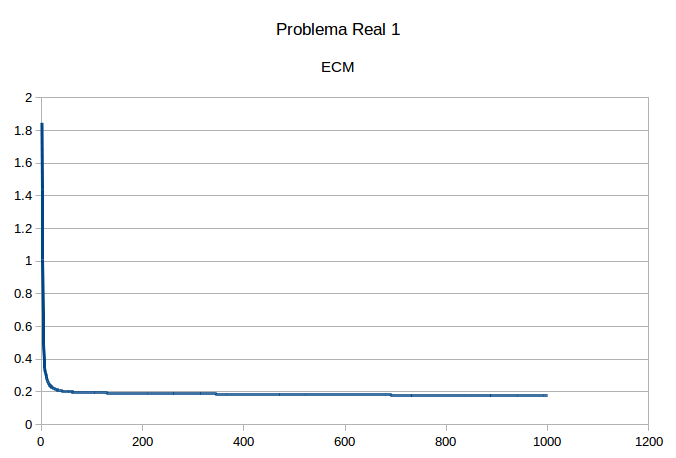
\includegraphics[width=160pt, height=100pt]{PR1h1.png}
				\caption{4 nodos,$\alpha$ = 0.01}
			\end{subfigure}\\
			\begin{subfigure}[t!]{\textwidth}
				\centering
				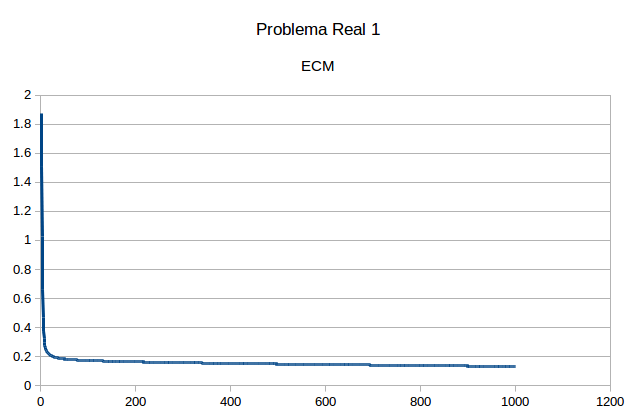
\includegraphics[width=160pt, height=100pt]{PR1h2.png}
				\caption{8 nodos, $\alpha$ = 0.01}
			\end{subfigure}\\
			\begin{subfigure}[t!]{\textwidth}
				\centering
				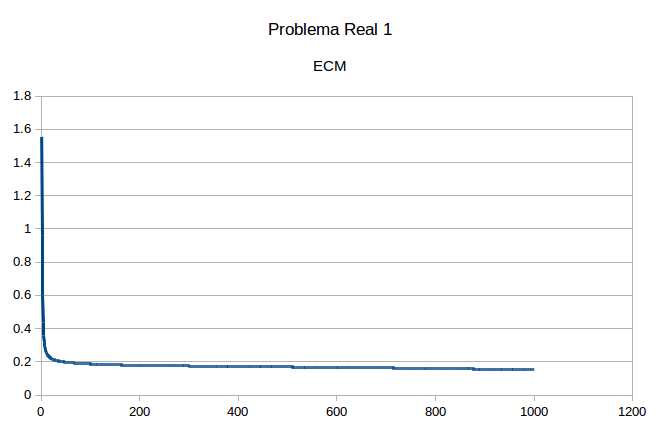
\includegraphics[width=160pt, height=100pt]{PR1h3.png}
				\caption{12 nodos, $\alpha$ = 0.01}
			\end{subfigure}
		\end{subfigure}
		\begin{subfigure}[t!]{0.5\textwidth}
			\begin{subfigure}[t!]{\textwidth}
				\centering
				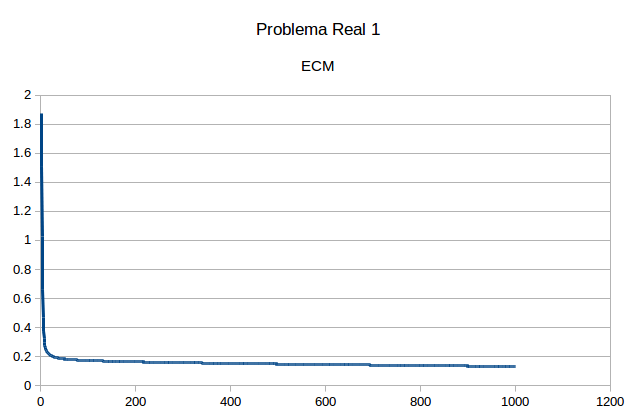
\includegraphics[width=160pt, height=100pt]{PR1h2.png}
				\caption{$\alpha$ = 0.01, 8 nodos}				
			\end{subfigure}
			\begin{subfigure}[t!]{\textwidth}
				\centering
				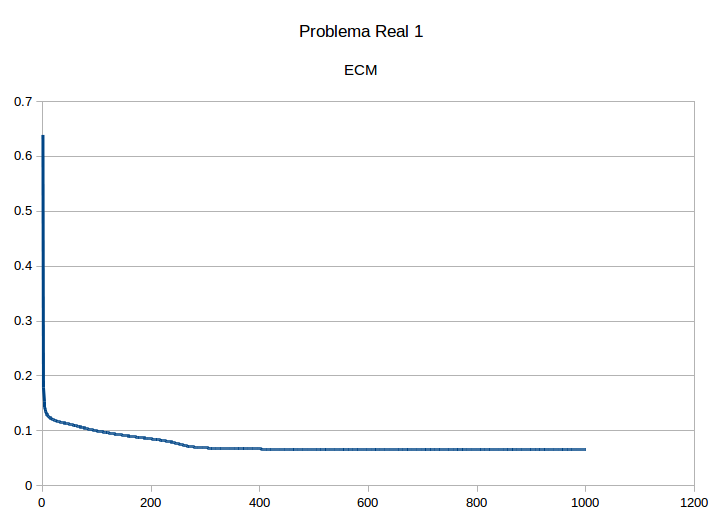
\includegraphics[width=160pt, height=100pt]{PR1a1.png}
				\caption{$\alpha$ = 0.1, 8 nodos}				
			\end{subfigure}
			\begin{subfigure}[t!]{\textwidth}
				\centering
				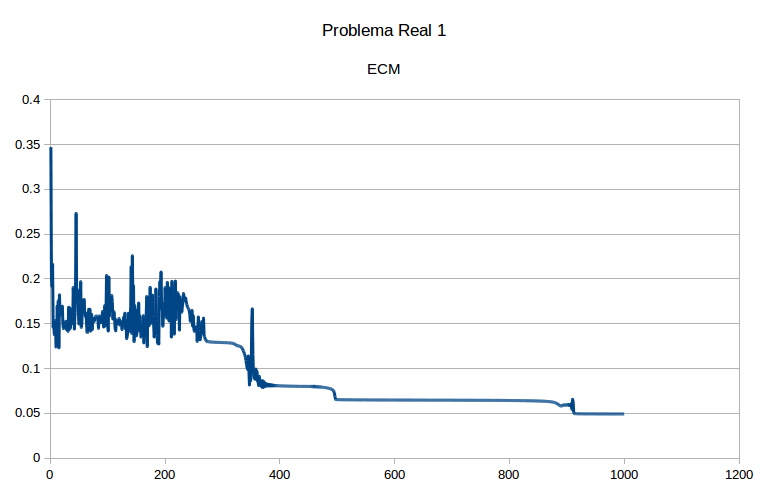
\includegraphics[width=160pt, height=100pt]{PR1a2.png}
				\caption{$\alpha$ = 0.5, 8 nodos}				
			\end{subfigure}
		\end{subfigure}
		\caption{%
			Gráficas de ECM para variaciones del número de neuronas (columna izquierda) y parámetro $\alpha$ (columna derecha).
		}%
		\label{fig:ECM_mosaic}
	\end{figure}
	
	Además, en el cuadro \ref{tab:pr1chart} podemos ver los porcentajes de acierto sobre los conjuntos de training y test para las variaciones de parámetros anteriores:
	
	\begin{table}[ht!]
		\centering
		\begin{tabular}{|l|l|l|l|}
			\hline
			\textbf{$\alpha$} & \textbf{\#Neuronas} & \textbf{ \%Acierto Training} & \textbf{\%Acierto Test} \\ \hline
			0.01& 4 & 97.34 & 98.10 \\ \hline
			0.01& 8 & 97.95 & 96.68 \\ \hline
			0.01& 12 & 97.54 & 96.20 \\ \hline
			0.1& 8 & 99.38 & 94.78 \\ \hline
			0.5& 8 & 99.38 & 92.89 \\ \hline
		\end{tabular}
		\caption{\% de acierto en entrenamiento y test con variación de parámetros.}
		\label{tab:pr1chart}
	\end{table}
	
	Como se puede comprobar, en las gráficas de ECM apenas existen diferencias, tienen un comportamiento muy similar y teóricamente correcto. Sí se puede observar que una tasa de aprendizaje demasiado alta produce fuertes oscilaciones en los pesos y consecuentemente en el ECM, por lo que preferiremos tasas de aprendizaje cercanas a cero, pero no demasiado pequeñas para que la convergencia no sea muy lenta. En esta práctica nuestro valor predilecto será $\alpha = 0.01$. Por otro lado se puede observar que, generalmente funciona mejor un número de nodos en la capa intermedia que sea menor o igual que el número de atributos de entrada y mayor o igual que el número de neuronas de salida. Los resultados cuando dicho número es estrictamente menor son muy similares a cuando es igual, si bien generalmente son mejores que cuando el número de neuronas de la capa oculta es mayor que el número de atributos de entrada y neuronas de salida.
	
	\subsection{Problema XOR}
	En la práctica 1 veíamos como el problema xor no se podía resolver con un perceptrón de una sola capa por no ser linealmente separable. Con el perceptrón multicapa si ha sido posible resolver este problema, si bien ha sido necesario modificar el archivo de muestras para añadir más muestras (simplemente se han replicado las cuatro muestras del problema hasta alcanzar un total de aproximadamente 500). Con este archivo (xor2.txt) se puede resolver completamente el problema en 1000 épocas con una tasa de acierto de 100 \%.
	
	\newpage
	\section{Tarea 3: predicción en problemas con más de dos clases.}
	
	En el apartado anterior, vimos como generalmente era preferible un $\alpha$ pequeño (elegimos $\alpha = 0.01$) y un número de neuronas en la capa intermedia que fuera menor o igual que el numero de atributos de entrada y mayor o igual que el número de neuronas de salida. Se han repetido dichos experimentos para el problema real 3 y los resultados se presentan en el cuadro \ref{tab:pr3chart}.	
	\begin{table}[ht!]
		\centering
		\begin{tabular}{|l|l|l|l|}
			\hline
			\textbf{$\alpha$} & \textbf{\#Neuronas} & \textbf{ \%Acierto Training} & \textbf{\%Acierto Test} \\ \hline
			0.01& 2 & 95.23 & 89.13 \\ \hline
			0.01& 4 & 96.19 & 100.00 \\ \hline
			0.01& 6 & 96.19 & 97.82 \\ \hline
			0.1& 4 & 97.14 & 97.82 \\ \hline
			0.5& 4 & 73.33 & 63.04 \\ \hline
		\end{tabular}
		\caption{\% de acierto en entrenamiento y test con variación de parámetros.}
		\label{tab:pr3chart}
	\end{table}
	
	Se reafirman las conclusiones obtenidas en el apartado anterior. Nuestro problema tiene 4 atributos y 3 neuronas de salida y los mejores resultados se producen con 4 neuronas en la capa oculta y una tasa $\alpha=0.01$. Se puede observar que una cantidad de neuronas inferior tanto al número de atributos de entrada como al número de neuronas de salida produce un resultado considerablemente peor, al igual que una tasa de aprendizaje demasiado alta.
	
	Las gráficas de ECM son completamente análogas a las del apartado anterior, produciéndose oscilaciones en la gráfica con $\alpha = 0.5$, por esa razón se ha decidido omitirlas y se muestra únicamente la gráfica correspondiente al mejor resultado:	
	\begin{figure}[h]
		\centering
		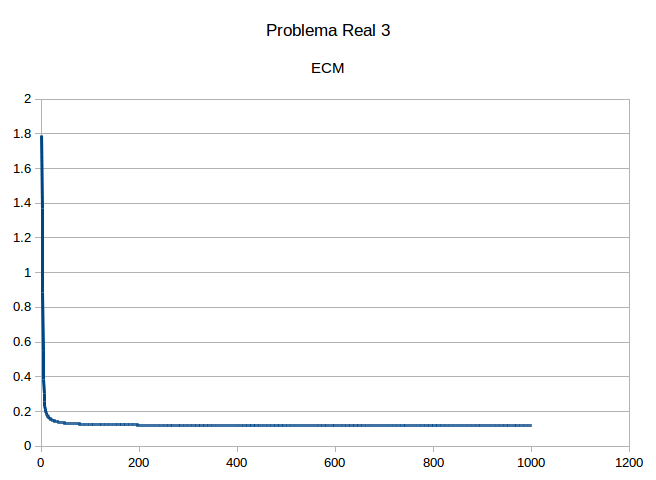
\includegraphics[scale=0.4]{PR3ECM.png}		
		\caption{ECM para el problema real 3. $\alpha = 0.01$, 4 neuronas en capa oculta}				
	\end{figure}

	\section{Tarea 4: Predicción en un problema complejo.}
	Para resolver este problema se han elegido los siguientes parámetros para el aprendizaje de la red:
	\begin{itemize}
		\item Conjunto de entrenamiento: $70\%$
		\item Conjunto de test: $30\%$
		\item Tasa de aprendizaje $\alpha = 0.01$.		
		\item Número de nodos de la capa oculta: $7$.
	\end{itemize}
	
	Con estos datos, se han obtenido los siguientes resultados:
	\begin{itemize}
		\item Tasa de acierto en el conjunto de \textbf{entrenamiento}: $80.2\%$
		\item Tasa de acierto en el conjunto de \textbf{test}: $60.3\%$
	\end{itemize}
	
	En la figura \ref{fig:p4} se puede observar la evolución del error cuadrático medio en función del número de la época de entrenamiento. Se puede observar que converge a un valor para el error cuadrático medio de $1.2$.
	
	\fimg{p4.png}{width=\textwidth}{Evolución del error cuadrático medio}{p4}
	
	Vemos que la tasa de acierto en ambos conjuntos no es muy elevada, sin ni siquiera acercarse al
	$90\%$. Esto se debe, principalmente, a cómo están distribuidos los parámetros utilizados para el entrenamiento de la red, es decir, el conjunto de atributos. Se han calculado las medias y las desviaciones estándar de todos los atributos del problema, obteniéndose para varios de ellos, medias y desviaciones típicas muy grandes, incluso del orden de $10^3$.
	
	Normalmente, la convergencia es más rápida si las medias de los atributos son cercanas a cero. Esto se debe a que, en caso de que esto no ocurra, el descenso por gradiente del algoritmo de \textit{backpropagation} hará zig-zag en lugar de tomar la dirección de máximo decrecimiento, obteniéndose una convergencia más lenta. 
	
	La convergencia también es más rápida si los valores son reescalados y tienen desviación estándar 1. Esto se debe a que, si reescalamos los valores de entrada, se balancea la tasa a la que los pesos conectados a los nodos de entrada aprenden.
	
	Por tanto, si se normalizan los datos haciendo que el conjunto de los mismos tenga media 0 y desviación típica 1, se obtendrá una convergencia más rápida, y por tanto mejores resultados para el mismo número de épocas.
	
	\section{Tarea 5: Normalización de los datos.}
	Para resolver este problema, se ha realizado un programa que normaliza los parámetros de los atributos de entrada. De esta manera, al restarle a cada atributo la media del conjunto y dividirlo por la desviación típica del mismo, obtenemos que el conjunto de los atributos adquiere una distribución de media $0$ y desviacion típica $1$. Se han utilizado los mismos parámetros que en la tarea anterior, con el fin de poder realizar un análisis comparativo:
	\begin{itemize}
		\item Conjunto de entrenamiento: $70\%$
		\item Conjunto de test: $30\%$
		\item Tasa de aprendizaje $\alpha = 0.01$.		
		\item Número de nodos de la capa oculta: $7$.
	\end{itemize}
	
	Con estos datos, se han obtenido los siguientes resultados:
	\begin{itemize}
		\item Tasa de acierto en el conjunto de \textbf{entrenamiento}: $99.6\%$
		\item Tasa de acierto en el conjunto de \textbf{test}: $94.3\%$
	\end{itemize}
	
	\fimg{p4norm.png}{width=\textwidth}{Evolución del error cuadrático medio}{p4norm}
	
	En la figura \ref{fig:p4norm} se puede observar la evolución del error cuadrático medio en función del número de la época de entrenamiento. 
	
	En este caso, se puede observar que la velocidad de convergencia es mucho mas rápida. El error desciende en todo momento, y aunque se puede notar que en las primeras épocas se ralentiza este descenso, finalmente parece converger a cero. 
	
	Si comparamos los resultados con el del apartado anterior, podemos confirmar que la normalización de los datos mejora notablemente la velocidad de convergencia, obteniéndose así unos resultados mucho mejores tanto para el conjunto de entrenamiento ($99.6\%$) como para el conjunto de test ($94.3\%$), frente a los valores anteriores, que eran de un $80.2\%$ para el conjunto de entrenamiento y de un $60.3\%$ para el conjunto de test.
	
	\section{Tarea 6: Predicción de datos no etiquetados.}
	Para realizar esta tarea, se ha realizado un programa que toma un fichero para entrenar la red y otro para clasificar, obteniéndose un fichero de salida con la clasificación obtenida. 
	Tras varias pruebas utilizando el fichero con los datos clasificados, se han elegido los siguientes parámetros para resolver este problema:
	\begin{itemize}
		\item Número de nodos de la capa intermedia: $5$.
		\item Valor de la tasa de aprendizaje $\alpha = 0.01$.
	\end{itemize}
	El fichero \textit{predicciones$\_$nnet.txt} se adjunta con la práctica.
	
\end{document}